% Copyright 2004 by Till Tantau <tantau@users.sourceforge.net>.
%
% In principle, this file can be redistributed and/or modified under
% the terms of the GNU Public License, version 2.
%
% However, this file is supposed to be a template to be modified
% for your own needs. For this reason, if you use this file as a
% template and not specifically distribute it as part of a another
% package/program, I grant the extra permission to freely copy and
% modify this file as you see fit and even to delete this copyright
% notice. 

\documentclass{beamer}
% Replace the \documentclass declaration above
% with the following two lines to typeset your 
% lecture notes as a handout:
%\documentclass{article}
%\usepackage{beamerarticle}

\usepackage[utf8x]{inputenc}
\usepackage[spanish]{babel}
\usepackage{verbatim}

% There are many different themes available for Beamer. A comprehensive
% list with examples is given here:
% http://deic.uab.es/~iblanes/beamer_gallery/index_by_theme.html
% You can uncomment the themes below if you would like to use a different
% one:
%\usetheme{AnnArbor}
%\usetheme{Antibes}
%\usetheme{Bergen}
%\usetheme{Berkeley}
%\usetheme{Berlin}
%\usetheme{Boadilla}
%\usetheme{boxes}
%\usetheme{CambridgeUS}
%\usetheme{Copenhagen}
%\usetheme{Darmstadt}
%\usetheme{default}
%\usetheme{Frankfurt}
%  \usetheme{Goettingen}
%\usetheme{Hannover}
%\usetheme{Ilmenau}
%\usetheme{JuanLesPins}
%\usetheme{Luebeck}
%\usetheme{Madrid}
%\usetheme{Malmoe}
%\usetheme{Marburg}
%\usetheme{Montpellier}
%\usetheme{PaloAlto}
%\usetheme{Pittsburgh}
%\usetheme{Rochester}
\usetheme{Singapore}
%\usetheme{Szeged}
%\usetheme{Warsaw}


\title{Automatización y Scripting}


\begin{document}

\begin{frame}
  \titlepage
\end{frame}





\begin{frame}{}
El shell de UNIX interpreta los comandos del usuario. Los comandos pueden ser :
\begin{itemize}
\item Escritos directamente 
\item Leidos desde un archivo llamado programa script del shell 
\end{itemize}
\\ \

Los scripts son interpretados, no compilados
\begin{itemize}
\item El shell lee los comandos desde el script linea por linea, y busca los comandos en el sistema.
\item Un programa compilado es generado por un compilador, y es un archivo ejecutable.
\end{itemize}

\end{frame}


\begin{frame}{}
Algunos de los shells más conocidos : 
\begin{itemize}
\item sh (Bourne Shell)
\item bash (Bourne Again shell)
\item csh (C shell)
\item tcsh (TENEX C)
\item ksh (Korn shell)
\end{itemize}
\\ \

Puede observar en su sistema GNU/Linux que shells tiene disponible con : \texttt{cat /etc/shells}


\end{frame}


\begin{frame}{}
Archivos leídos por BASH : 

\texttt{ /etc/profile}

\texttt{~/.bash\_profile, ~/.bash\_login or ~/.profile }

\texttt{~/.bash\_logout (leído al salir) }

\end{frame}


\begin{frame}{}
\textbf{Escribiendo un script en BASH }
\begin{itemize}
\item Un programa script es un archivo de texto.
\item La primer línea del archivo debe ser : \texttt{\#!/bin/bash}
\item Debe tener permiso de ejecución (o ser ejecutado explicitamente con un shell).
\item Se sugiere dar un nombre acorde a lo que el script intenta realizar.
\item \textbf{No utilice nombres de programas existentes para no crear confusion}
\item Generalmente se suele colocar la extensión .sh al nombre del script
\end{itemize}

\end{frame}

\begin{frame}{}
\textbf{Ejecutando un script en BASH }
\begin{itemize}
\item El script debe ser copiado dentro de un directorio de PATH; o
\item debe ser ejecutado con la ruta relativa o completa. Ej. : \texttt{./script.sh}
\item Tambien puede ser ejecutado explicitamente por un shell. Ejemplo : \texttt{bash script.sh}
\end{itemize}

\end{frame}

\begin{frame}{}
\textbf{Algunas prácticas al escribir scripts }
\begin{itemize}
\item Se aconseja explicitamente indicar el shell con \#!
\item Deberia contar con al menos dos tipos de comentarios :
\begin{enumerate}
\item Un comentario al principio del programa script explicando a los usuarios que HACE el script.
\item Comentarios en el código, ya que no somos las únicas personas que leeremos el script 
(los administradores suelen ejecutar y modificar scripts escritos por otros administradores)
\end{enumerate}
\end{itemize}

\end{frame}


\begin{frame}{}
\textbf{Ejemplo de un script escrito en BASH }

\begin{center}
 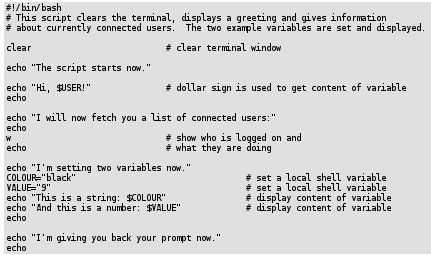
\includegraphics{script2.png}
 % redireccionamiento.gif: 502x248 pixel, 72dpi, 17.71x8.75 cm, bb=0 0 502 248
\end{center}

\end{frame}

\begin{frame}{}
Bibliografía : 
\begin{itemize}
\item man bash
\item Libro Bash Guide for Beginners, de Machtelt Garrels 
\item Libro Advanced Bash-Scripting Guide, de Mendel Cooper
\end{itemize}

Ambos libros están disponibles en varios formatos diferentes en :

Bibliografía suplementaria sugerida : 
\begin{itemize}
\item Libro El Entorno De Programacion Unix, de Kernighan, y Rob Pike
\end{itemize}

\end{frame}



\end{document}


